\documentclass[letterpaper,12pt]{article}
\usepackage[T1]{fontenc}
\usepackage{mathptmx}

% unit definition
\usepackage{siunitx}
% \sisetup{load-configurations = abbreviations}
\DeclareSIUnit\inch{in}
\DeclareSIUnit\ft{ft}
\DeclareSIUnit\Rank{^{\circ} R}
\DeclareSIUnit\Faren{^{\circ} F}
\DeclareSIUnit\lbm{lb_{m}}
\DeclareSIUnit\lbf{lb_{f}}
\DeclareSIUnit\torr{Torr}
\DeclareSIUnit\gallon{gal}
\DeclareSIUnit\slug{slug}
\DeclareSIUnit\knots{kts}
\DeclareSIUnit\miles{mi}


% hyperlink formatting
\usepackage{hyperref}
\hypersetup{
    colorlinks=true,
    linkcolor=red,
    urlcolor=purple,
    citecolor=blue
}


% Other general packages
\usepackage{setspace}
\usepackage{graphicx}
\usepackage{float}
\usepackage{amsmath}
\usepackage{amssymb}
\usepackage{tabto}
\usepackage{booktabs, tabularx}
\usepackage{enumitem}
\usepackage{gensymb}
\usepackage{cancel}
\usepackage{tikz}
\usepackage{pgfplots}
\usepackage{appendix}
\usepackage[labelfont=bf, font={normalsize,stretch=1}]{caption}
\usepackage[letterpaper, margin=1.0in]{geometry}
\usepackage[utf8]{}
\usepackage{indentfirst}
\setlength{\parindent}{0.25in}

%Heading format
\usepackage{titlesec}
\titleformat*{\section}{\normalsize\bfseries}
\titleformat*{\subsection}{\normalsize\bfseries}
\titleformat*{\subsubsection}{\normalsize\bfseries}

%Page Numbers
\usepackage{fancyhdr} 
\pagestyle{fancy}
\fancyhf{}
\fancyheadoffset{0cm}
\renewcommand{\headrulewidth}{0pt} 
\renewcommand{\footrulewidth}{0pt}
\fancyhead[R]{\thepage}
\pagenumbering{arabic}

%listings package for code
\usepackage{listings}
\usepackage{xcolor}

% bibliography formatting
\usepackage{etoolbox}
\patchcmd{\thebibliography}{\section*{\refname}}{}{}{}
\setstretch{2}

% color definitions
\definecolor{dblue}{HTML}{145680}
\definecolor{dred}{HTML}{801414}
\definecolor{dgreen}{HTML}{148014}
\definecolor{bgcode}{rgb}{0.95,0.95,0.95}
\definecolor{codegreen}{rgb}{0,0.6,0}
\definecolor{codegray}{rgb}{0.5,0.5,0.5}
\definecolor{codepurple}{rgb}{0.58,0,0.82}
\definecolor{backcolour}{rgb}{0.95,0.95,0.92}

\lstdefinestyle{mystyle}{
    backgroundcolor=\color{backcolour},
    commentstyle=\color{codegreen},
    keywordstyle=\color{magenta},
    numberstyle=\tiny\color{codegray},
    stringstyle=\color{codepurple},
    basicstyle=\ttfamily\footnotesize,
    breakatwhitespace=false,
    breaklines=true,
    captionpos=b,
    keepspaces=true,
    numbers=left,
    numbersep=5pt,
    showspaces=false,
    showstringspaces=false,
    showtabs=false,
    tabsize=2
}
\lstset{style=mystyle}

\pgfplotsset{compat=1.17}


\title{AE484 Assignment 3}
\author{George Petrov}
\date{February 21, 2022}

\begin{document}

\maketitle
\begin{singlespace}
\section{Symmetric and Cambered Airfoil Analysis}
\textbf{Note:}I have exported all of the polar's data from XLR5 then made python script to plot this data. All of the code will be attached at the bottom of the homework.
\subsection{Part (a)}
Plot of the coefficient of lift across different angles of attack can be seen below. The NACA 0012 airfoil is in blue and the NACA 4412 is in red.
\begin{figure}[H]
        \centering
        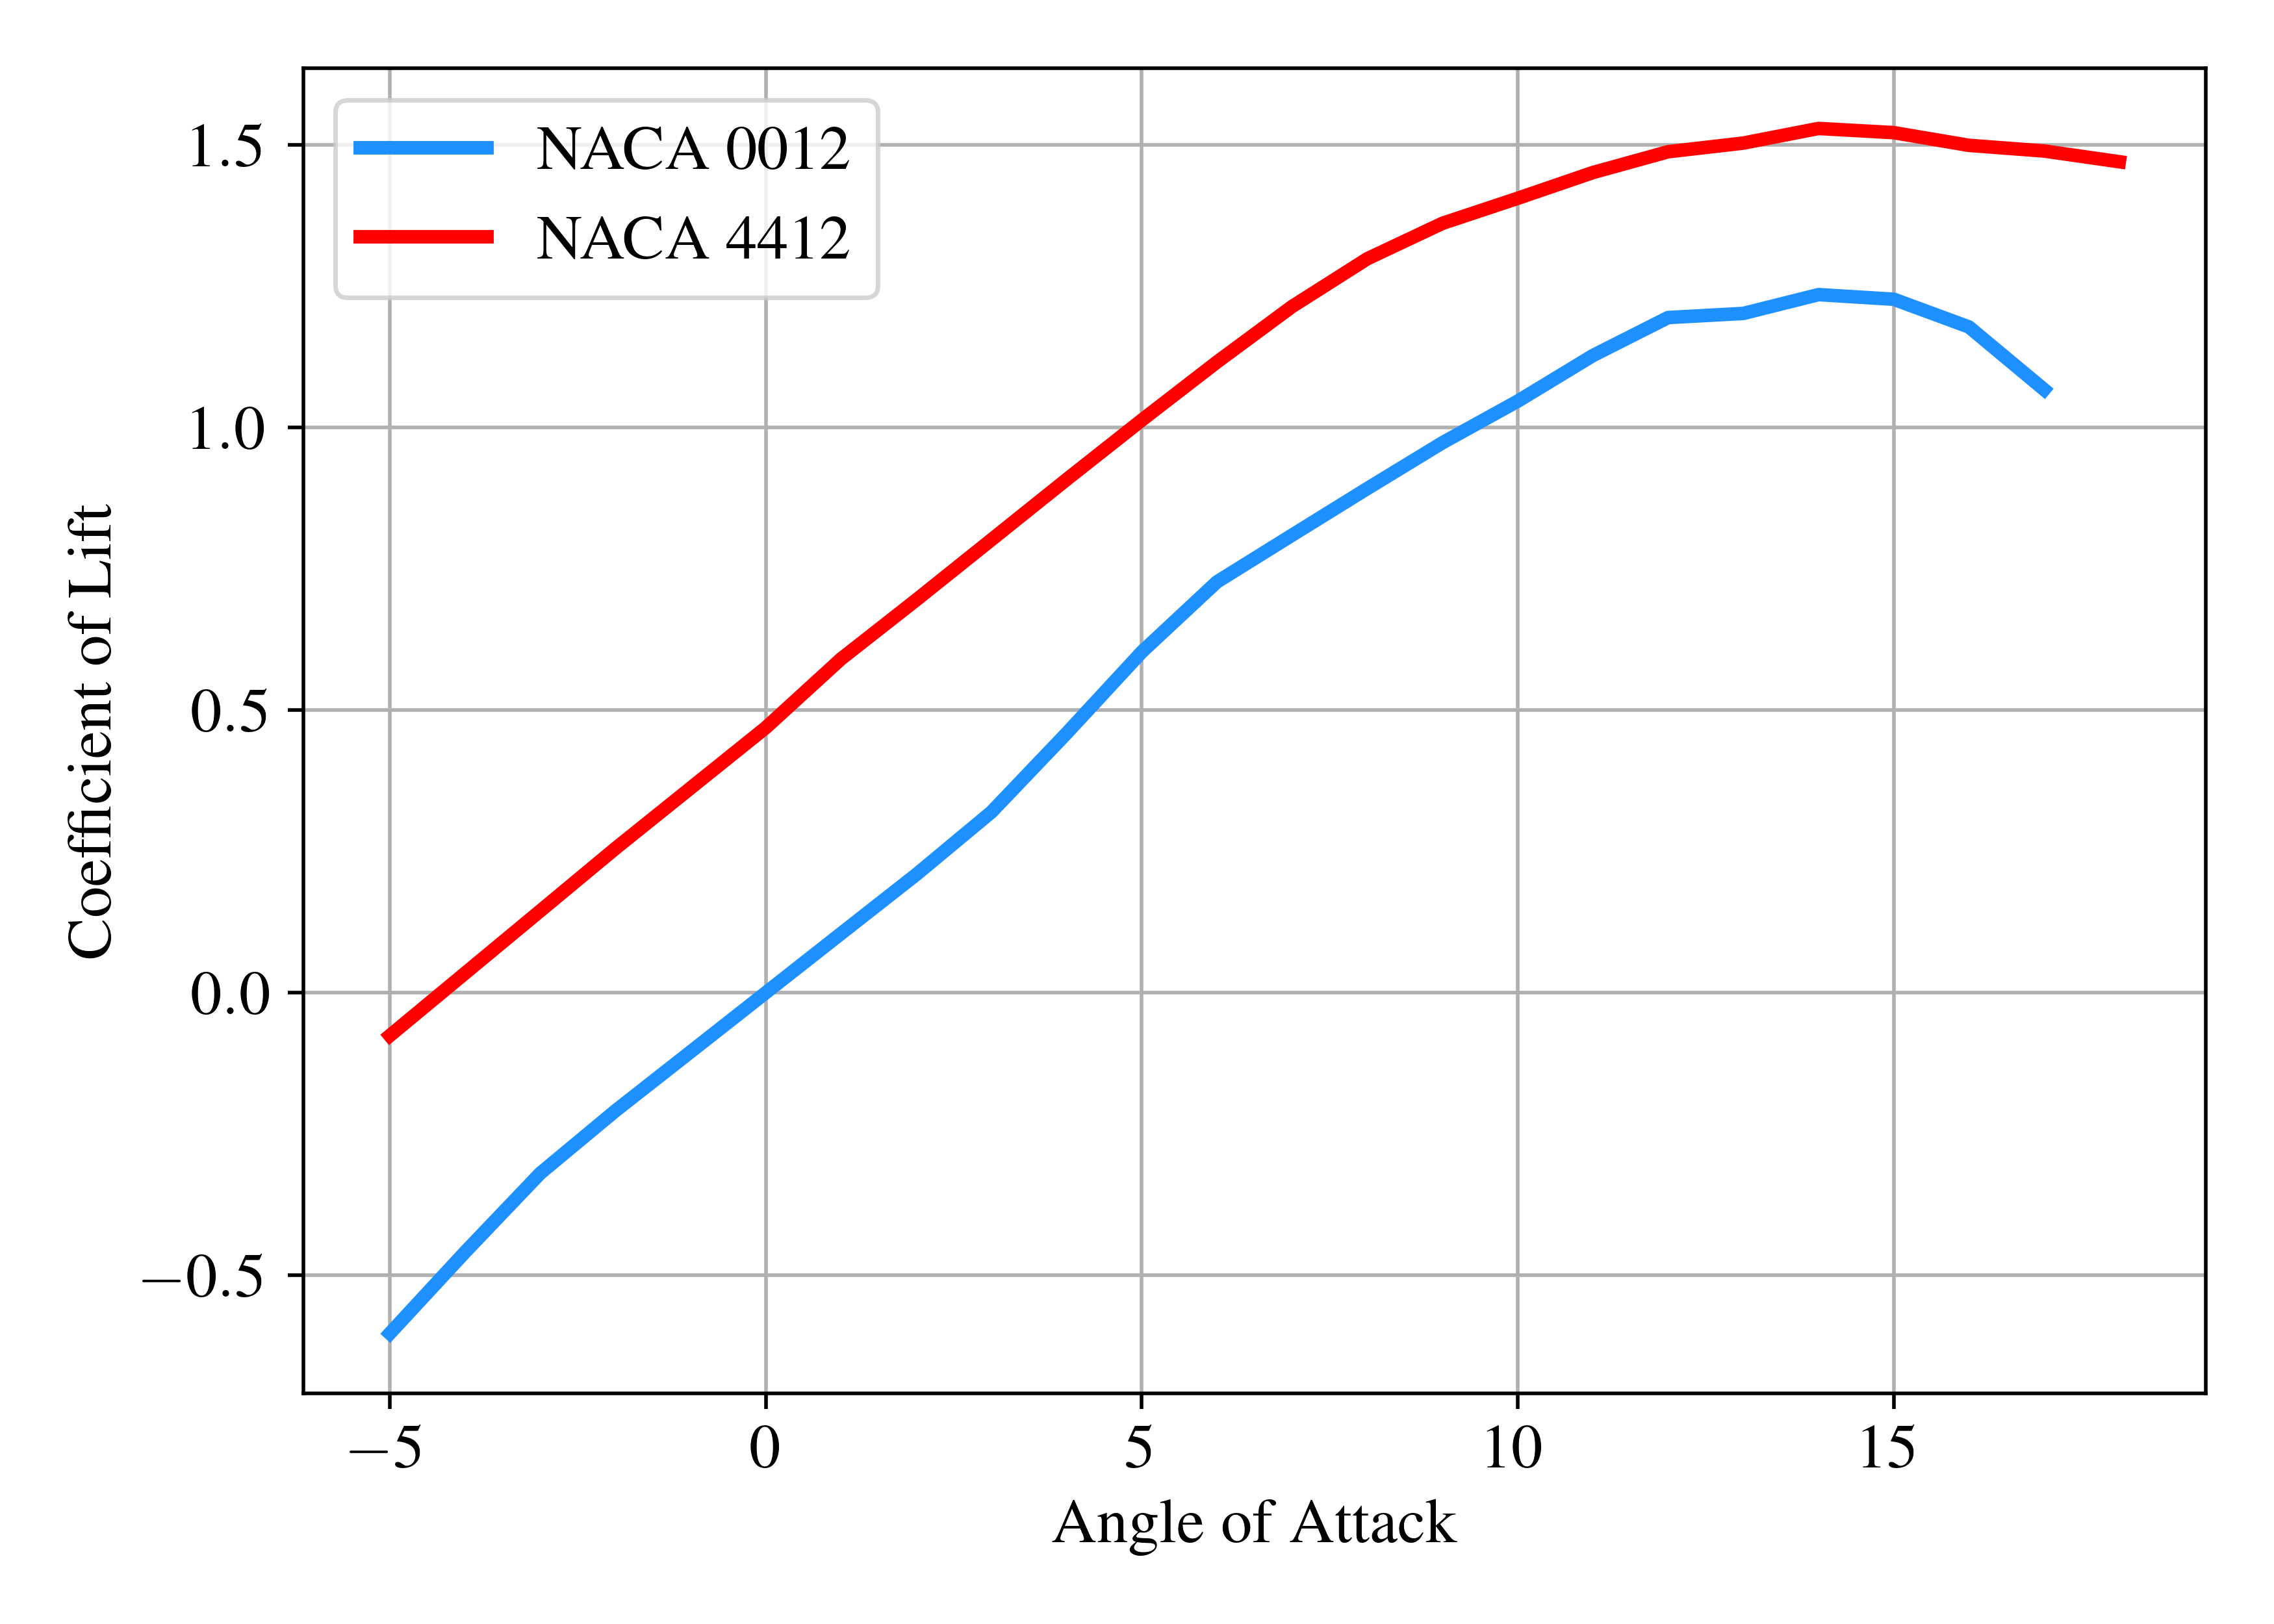
\includegraphics[width=.7\textwidth]{homeworks/homework3/george/plots/problem1_a.png}
        \caption{\textbf{$C_l$ vs. $\alpha$}}
        \label{fig:1a}
\end{figure}
\subsection{Part (b)}
Plot of the coefficient of drag across different angles of attack can be seen below.
\begin{figure}[H]
        \centering
        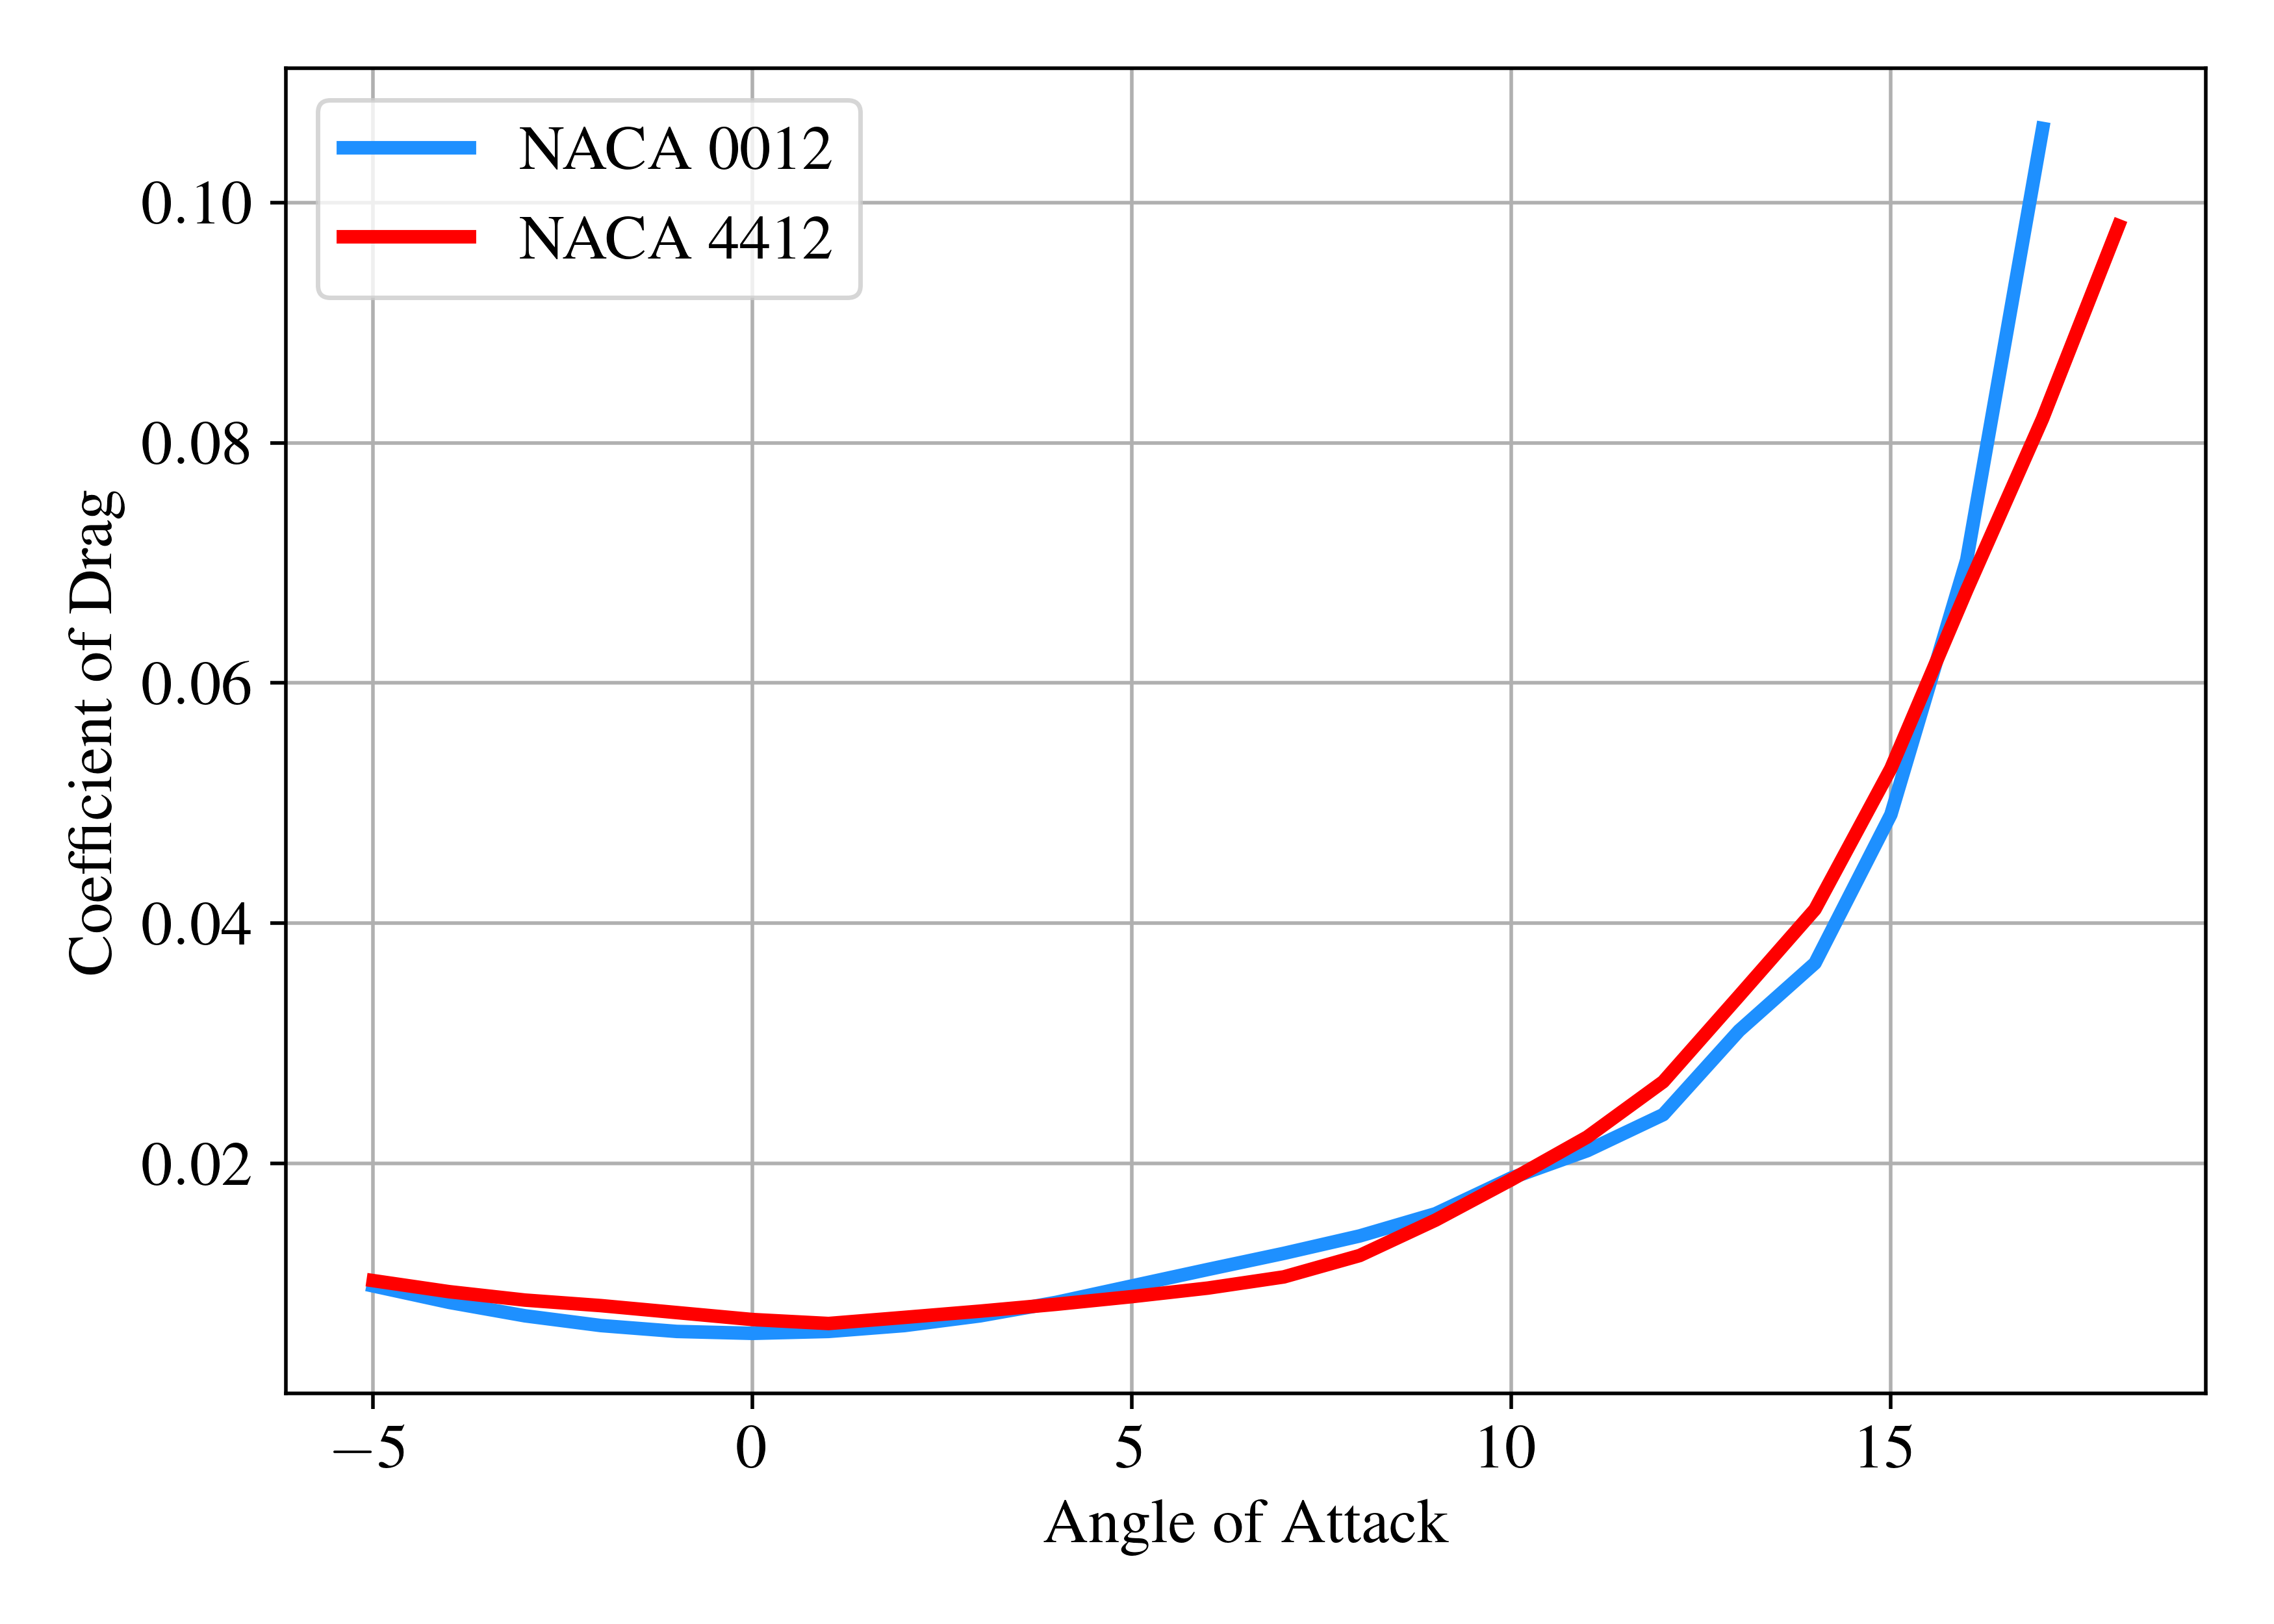
\includegraphics[width=.7\textwidth]{homeworks/homework3/george/plots/problem1_b.png}
        \caption{\textbf{$C_d$ vs. $\alpha$}}
        \label{fig:1b}
\end{figure}
\subsection{Part (c)}
Plot of the coefficient of lift vs. coefficient of drag can be seen below.
\begin{figure}[H]
        \centering
        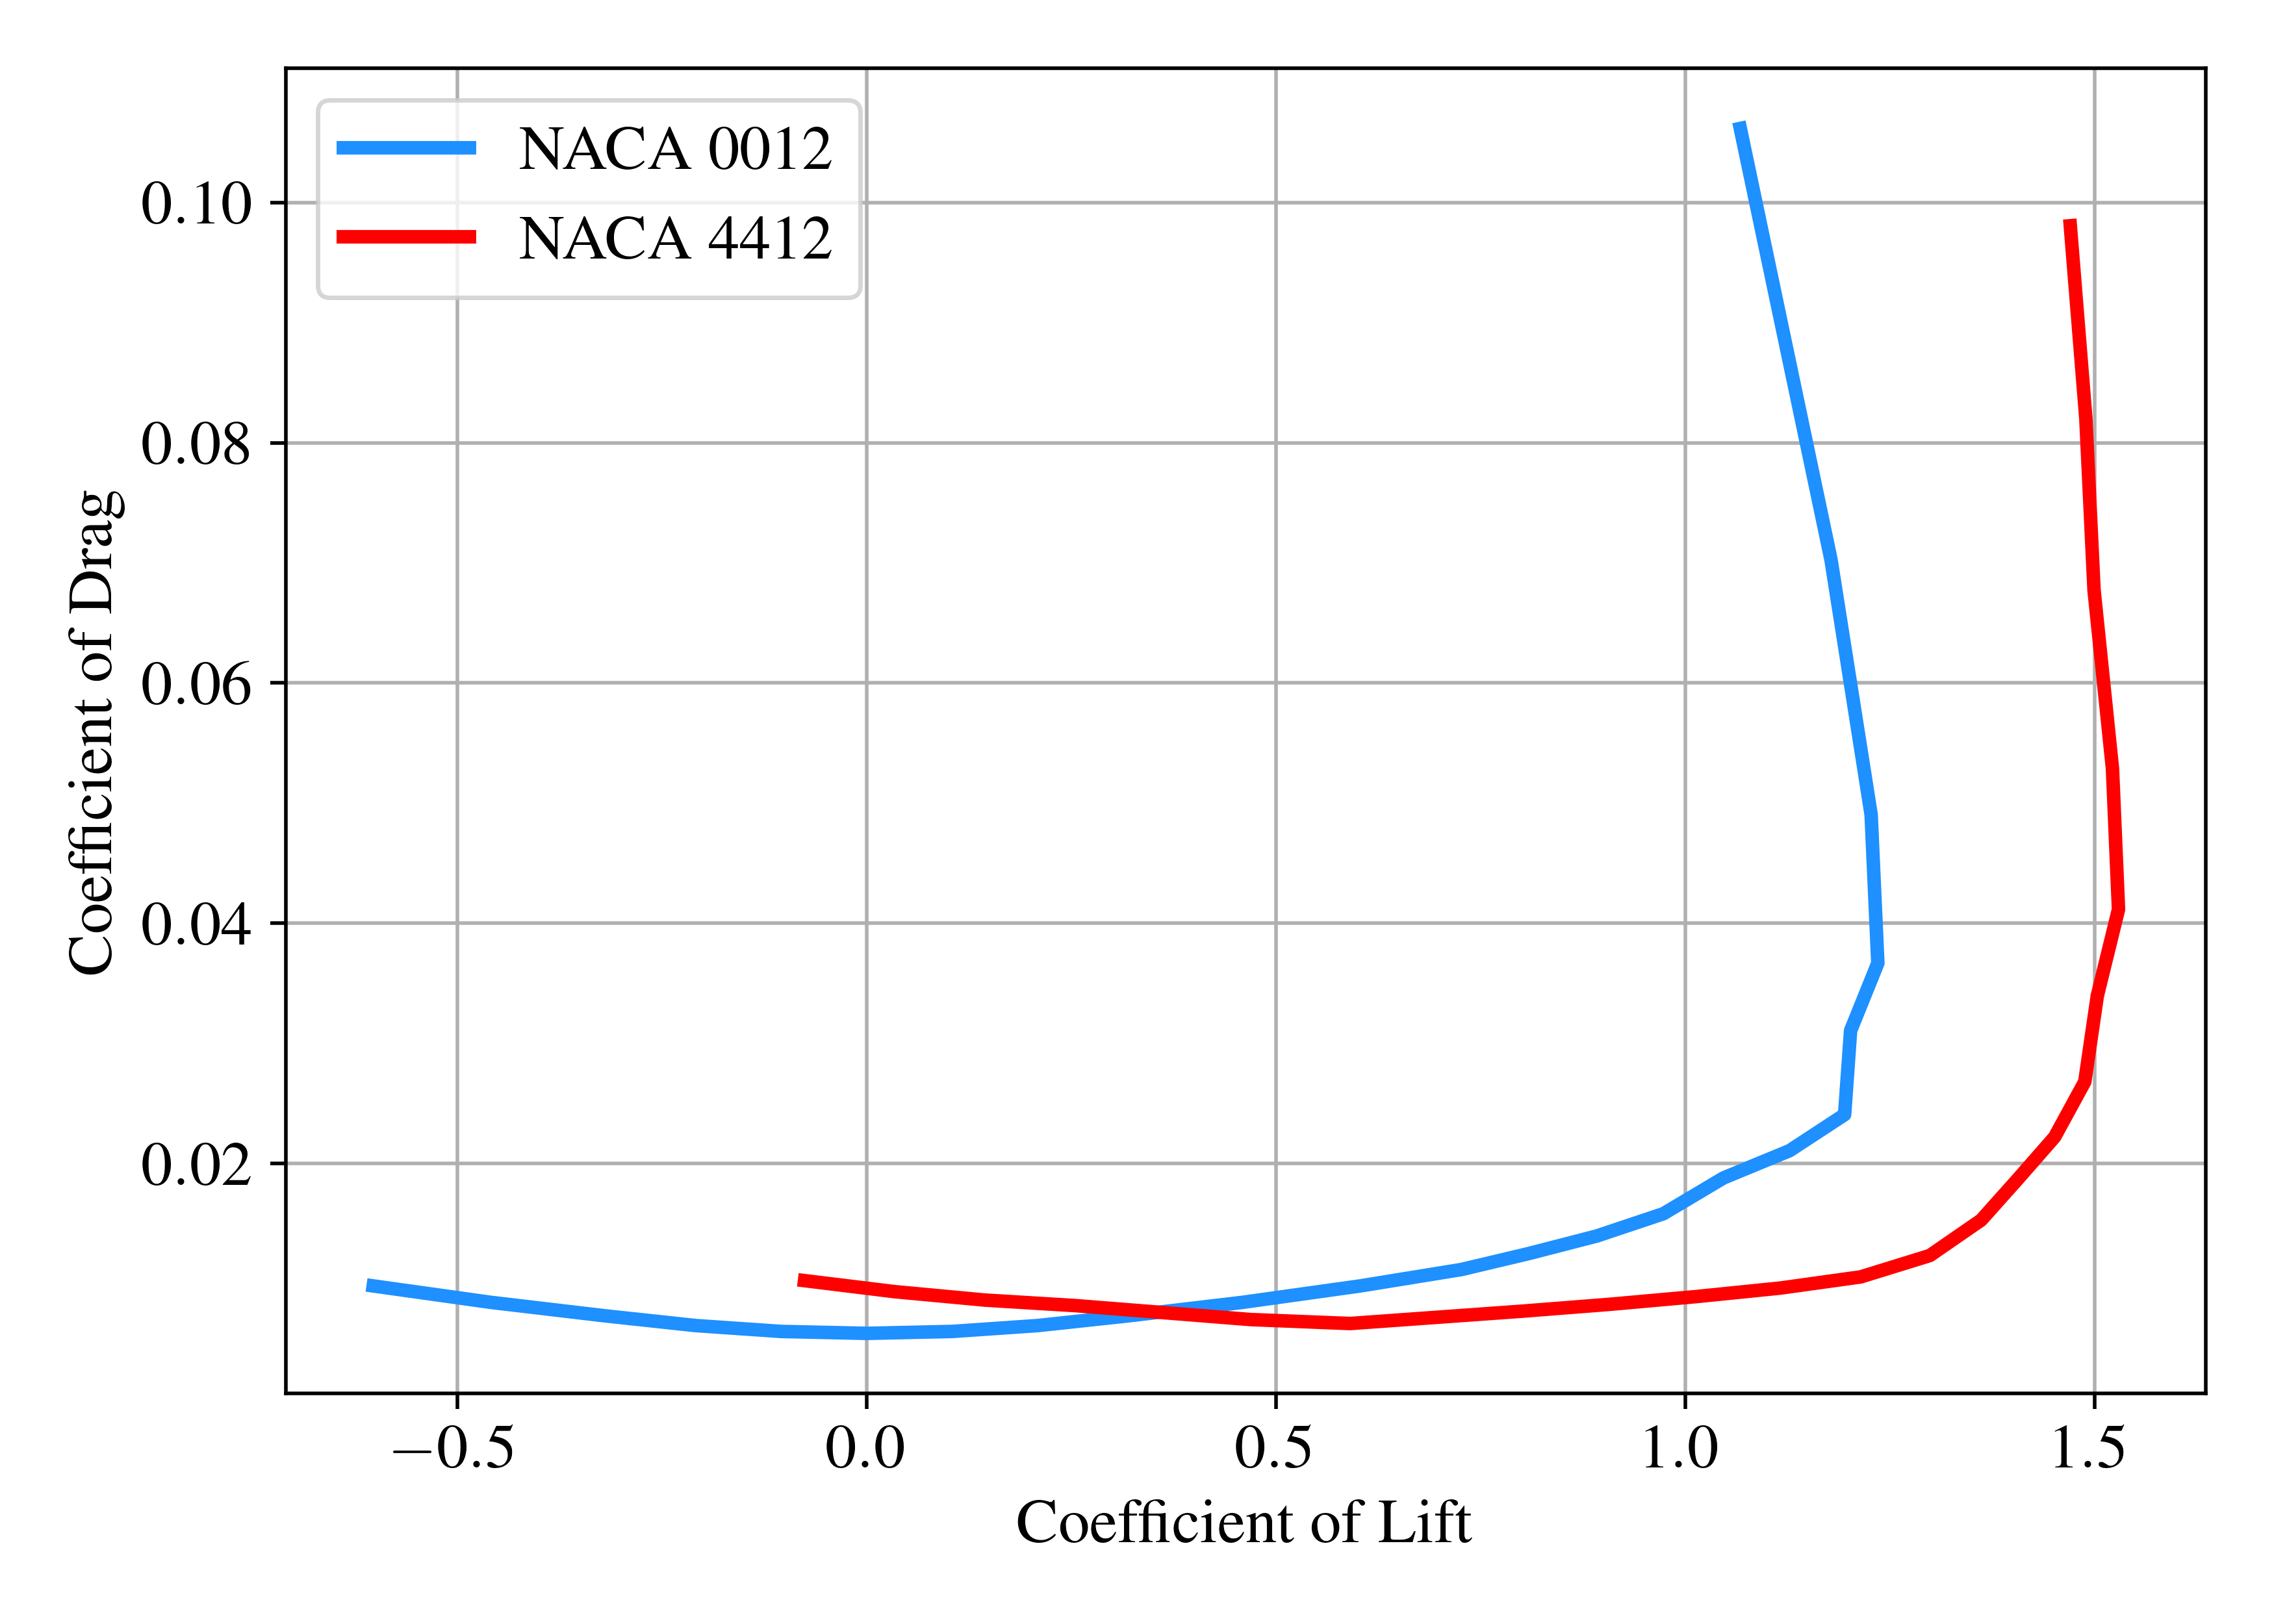
\includegraphics[width=.7\textwidth]{homeworks/homework3/george/plots/problem1_c.png}
        \caption{\textbf{$C_l$ vs. $C_d$}}
        \label{fig:1c}
\end{figure}
\subsection{Part (d)}
The different between the NACA 0012 and 4412 is their camber. The 0012 being a symmetric airfoil, while the 4412 being decently cambered. 

The difference can be seen in the Figure \ref{fig:1a}. In this plot, the symmetric airfoil only starts to create lift after the angle of attack is above 0 degrees. While the cambered airfoil creates lift at around -4 degrees. What is also interesting is that they still both stall at around the same angle of attack of 15 degrees. The lift coefficient of the 4412 is always much larger no matter the angle of attack which is expected due to its cambered nature. 

In Figure \ref{fig:1b}, we can see that their drag coefficients are largely the same no matter what the angle of attack is. At the end, the start to separate slightly where the 0012 has slightly larger drag.
For the plot of the coefficient of lift vs coefficient of drag plot, figure \ref{fig:1c}, we can see that the 4412 cambered airfoil is significantly more efficient in creating lift while keeping a similar drag profile to the 0012. 

A cambered wing offers more lift for no loss of drag. Yet, the NACA 0012 is still used in a number of tail stabilizers since it is symmetric.
\section{Finite Wing Analysis}
\subsection{Part (a)}
\subsubsection{i.}
The wings coefficient of lift at 6 and 12 degrees can be seen in the Table \ref{table:2ai} below.

    \begin{table}[H]
    \centering
        \begin{tabular}{|c|c|c|c|c|} % set column nums and width
            \hline \textbf{Angle of Attack ($\alpha$)} & \textbf{Coefficient of Lift ($C_L$)} \\ \hline % column headers
            6$\degree$ & 0.449725 \\ \hline
           12$\degree$ & 0.941413 \\ \hline
        \end{tabular}
        \label{table:2ai}
    \end{table}

    
\subsubsection{ii.}
Below are sceenshots of the finite wing model with the coefficient of pressure contour, the lift generation, and the streamlines of the flow are shown at both an angle of attack of 6 and 12 degrees.
\begin{figure}[H]
        \centering
        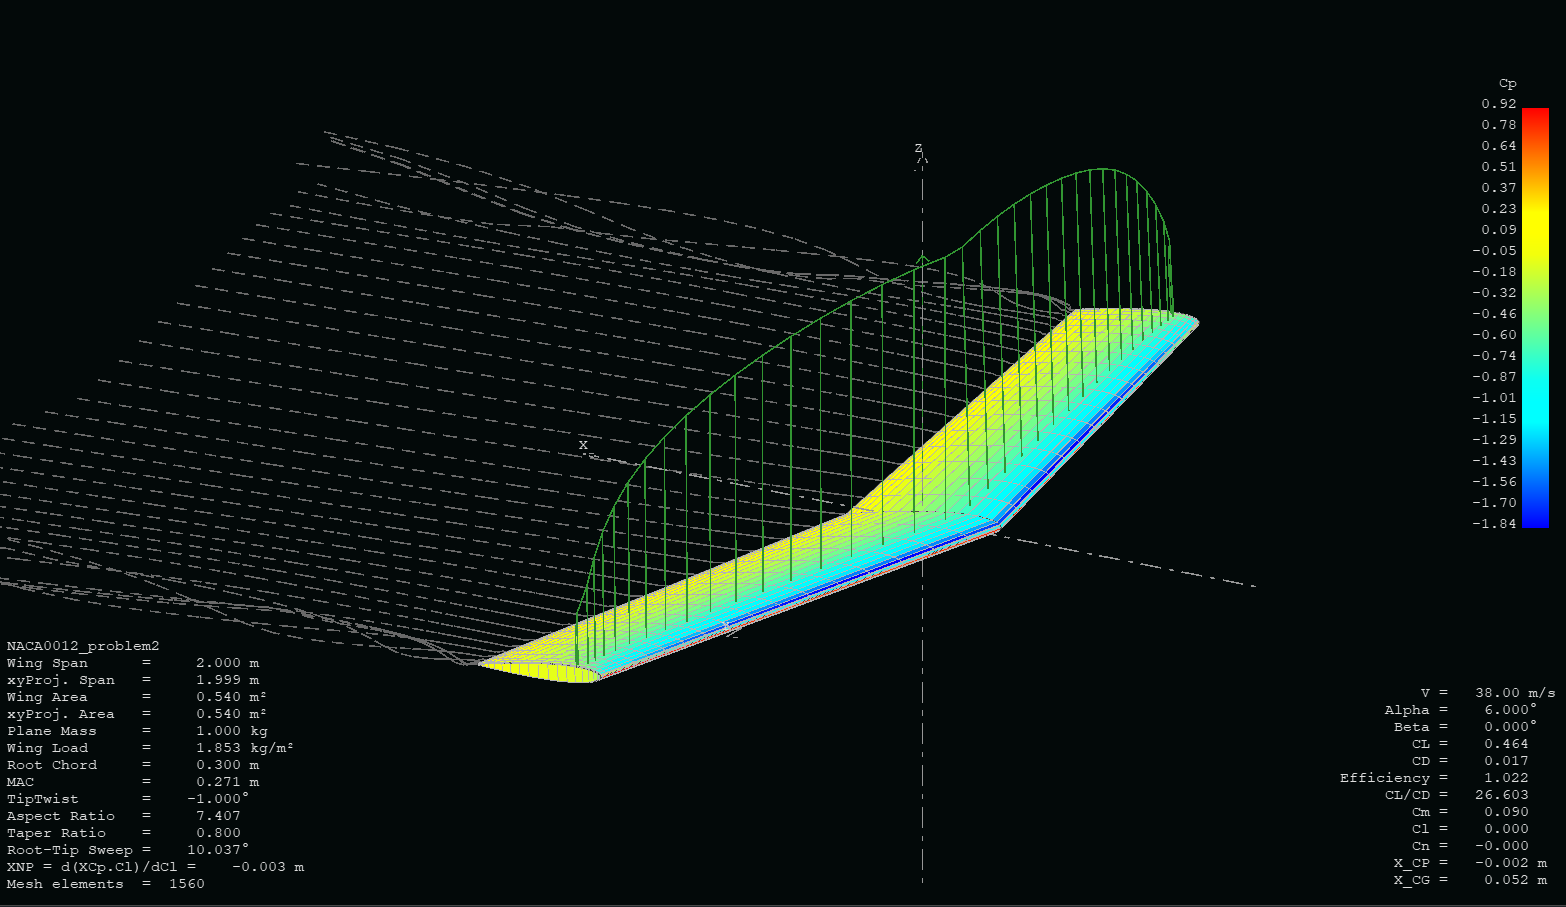
\includegraphics[width=1\textwidth]{homeworks/homework3/george/plots/problem2_b_6.PNG}
        \caption{\textbf{Contour $C_p$ mapping, $C_L$, and Streamlines at 6$\degree$}}
        \label{fig:2bii6}
\end{figure}
\begin{figure}[H]
        \centering
        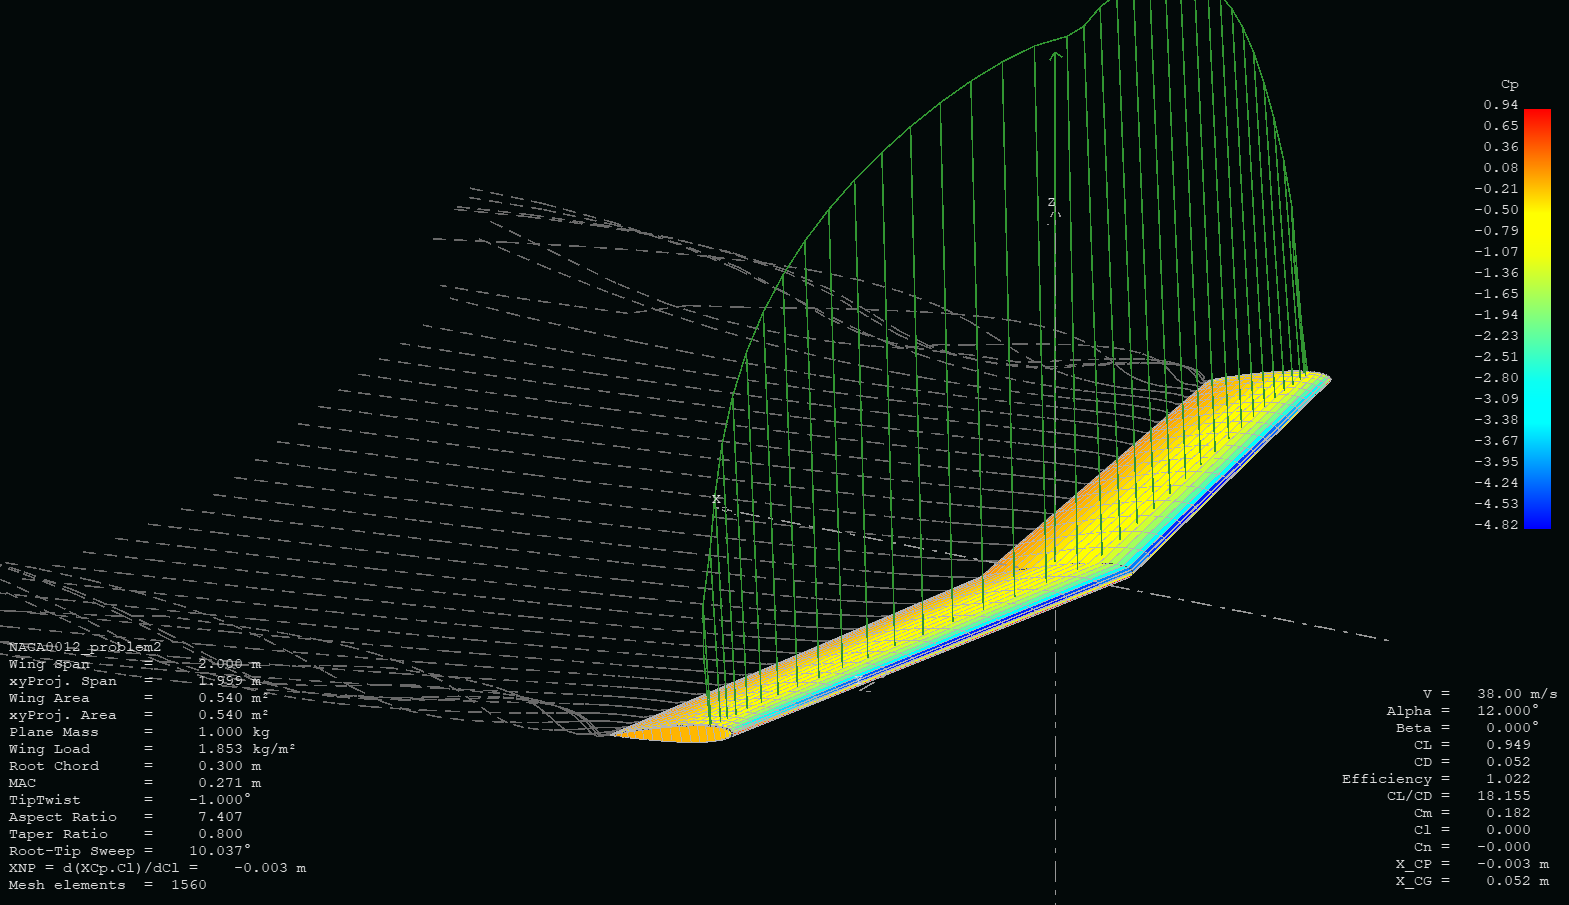
\includegraphics[width=1\textwidth]{homeworks/homework3/george/plots/problem2_b_12.PNG}
        \caption{\textbf{$C_p$ Contour , Lift, and Streamlines at 12$\degree$}}
        \label{fig:2bii12}
\end{figure}
\subsubsection{iii.}
Below, in Table \ref{table:2aiii}, the location of the coefficient of pressure load point and location of the center of gravity is shown for the angles of attack of 6 and 12 degrees. These distances are referenced from the tip of the wing.
\begin{table}[H]
    \centering
        \begin{tabular}{|c|c|c|c|c|} % set column nums and width
            \hline \textbf{Angle of Attack ($\alpha$)} & \textbf{$X_{cp}$} & \textbf{$X_{cg}$} \\ \hline % column headers
            6$\degree$ & 0.154 m & .204 m \\ \hline
           12$\degree$ & 0.152 m & .204 m \\ \hline
        \end{tabular}
        \label{table:2aiii}
    \end{table}
\subsection{Part (b)}
The neutral point for the wing is found to be \textbf{0.152 m} from the front of the wing.

\section{Flying Wing Analysis}
\subsection{Part (a)}
In order to observe whether the slope of the coefficient of moment vs angle of attack is positive or negative, it was plotted.

As we can see above in Figure \ref{fig:3ai}, the slope is very slightly negative.
\subsection{Part (b)}
\end{singlespace}
\end{document}